\documentclass[12pt]{article}
\usepackage[utf8]{inputenc}
\usepackage{graphics}
\usepackage{float}


\begin{document}
\section*{Supplementary Figures}

\noindent\textbf{Fig. S1.} Restricting set of studies to longer follow-up lengths

\begin{figure}[H]
    \centering
    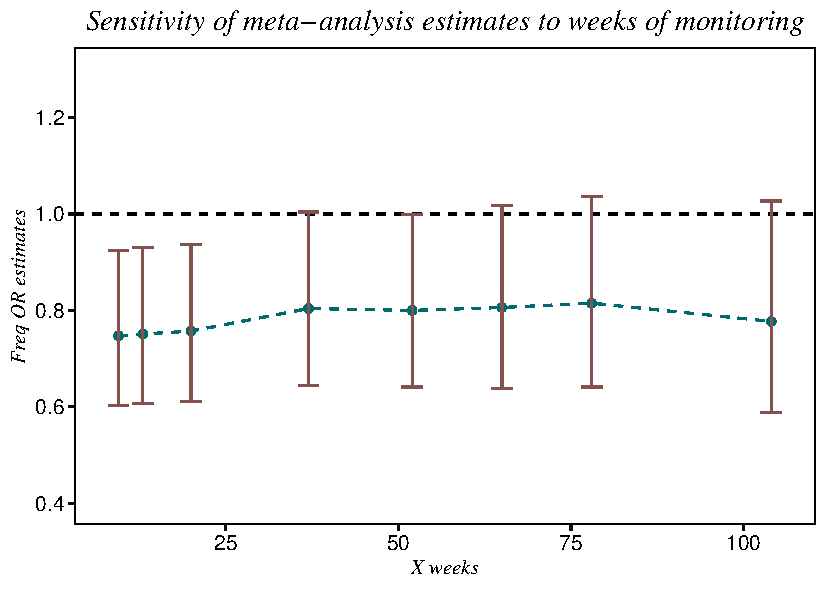
\includegraphics{figures/ma-week-plot.pdf}
\end{figure}

\noindent\fontsize{10}{10}\selectfont Notes: This figure presents the odds ratio estimated by the frequentist meta-analysis model with studies shorter than X weeks removed. Each point is the frequentist OR estimate, and the bars represent the 95\% Confidence Interval for each estimate. All 18 studies in the main sample are included for X = 9.5 weeks, and 4 studies are included for X = 104 weeks (2 years).

\newpage	
\noindent\textbf{Fig. S2.} Diarrhea effect estimates and compliance rates across included and excluded studies
\begin{figure}[H]
    \centering
    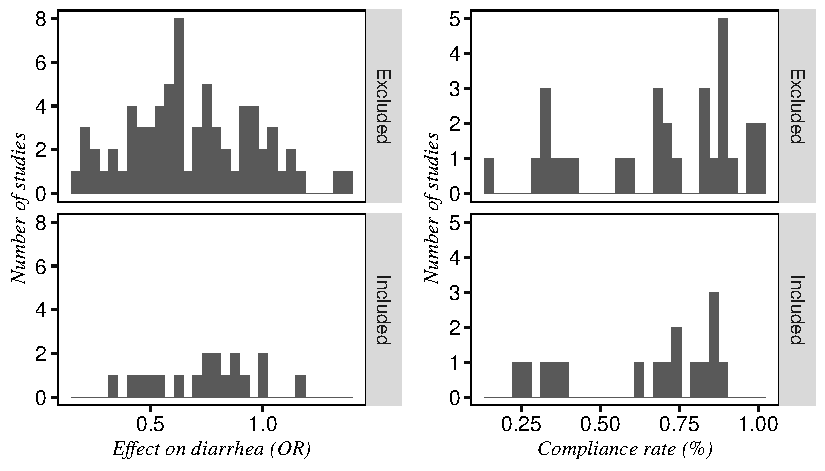
\includegraphics{figures/fig-compliance-diarr-hist.pdf}
\end{figure}
\noindent\hspace{1.0in}(A)
\noindent\hspace{3.0in}(B)\par

\vspace{\baselineskip}

\noindent\fontsize{10}{10}\selectfont Notes:  Figure (A) presents the diarrhea effect size across included (bottom panel) and excluded (top panel) studies. Figure (B) presents the compliance rate across included (bottom panel) and excluded (top panel) studies.



\newpage
\noindent\textbf{Fig. S3.} Funnel plot to examine publication bias

\begin{figure}[H]
    \centering
    \resizebox{\textwidth}{!}{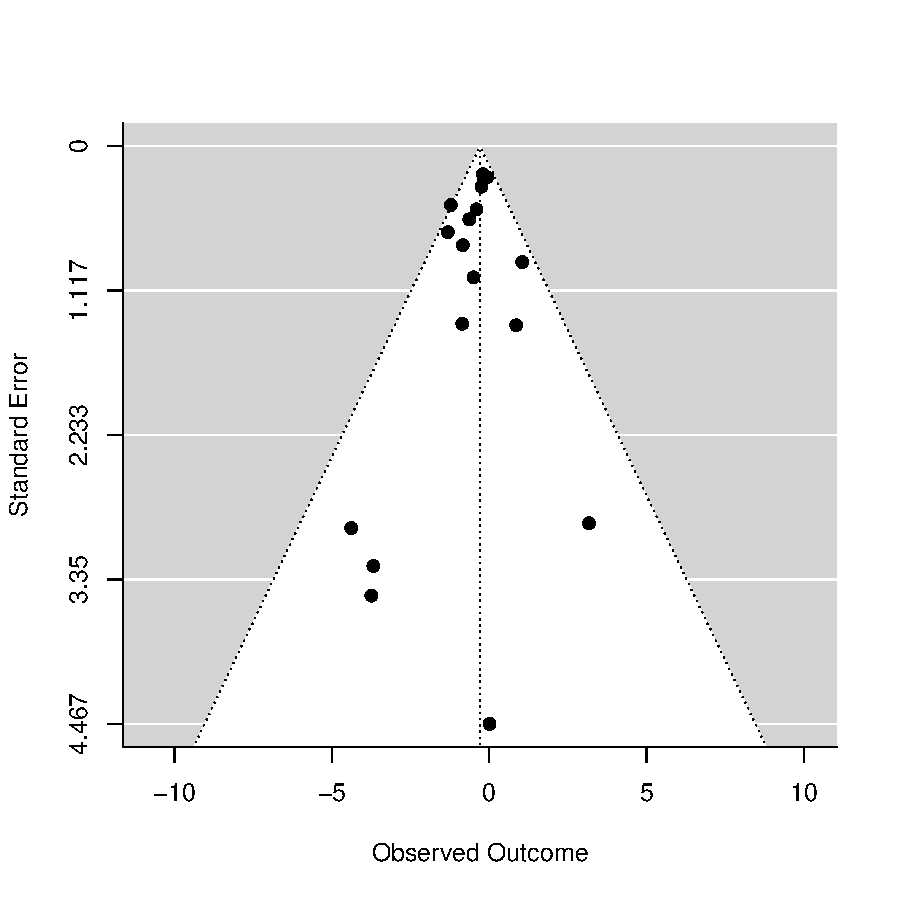
\includegraphics{figures/funnel.pdf}}
\end{figure}

\noindent\fontsize{10}{10}\selectfont Notes: This figure presents a funnel plot. Symmetry on either side of the vertical line (representing the overall effect) suggests that publication bias is not present. Results for funnel asymmetry test are reported in Materials and Methods, Section 5.

\newpage
\noindent\textbf{Fig. S4.} Funnel plot for all diarrhea interventions and chlorine diarrhea intervntions
\begin{figure}[H]
    \centering
     \resizebox{11cm}{!}{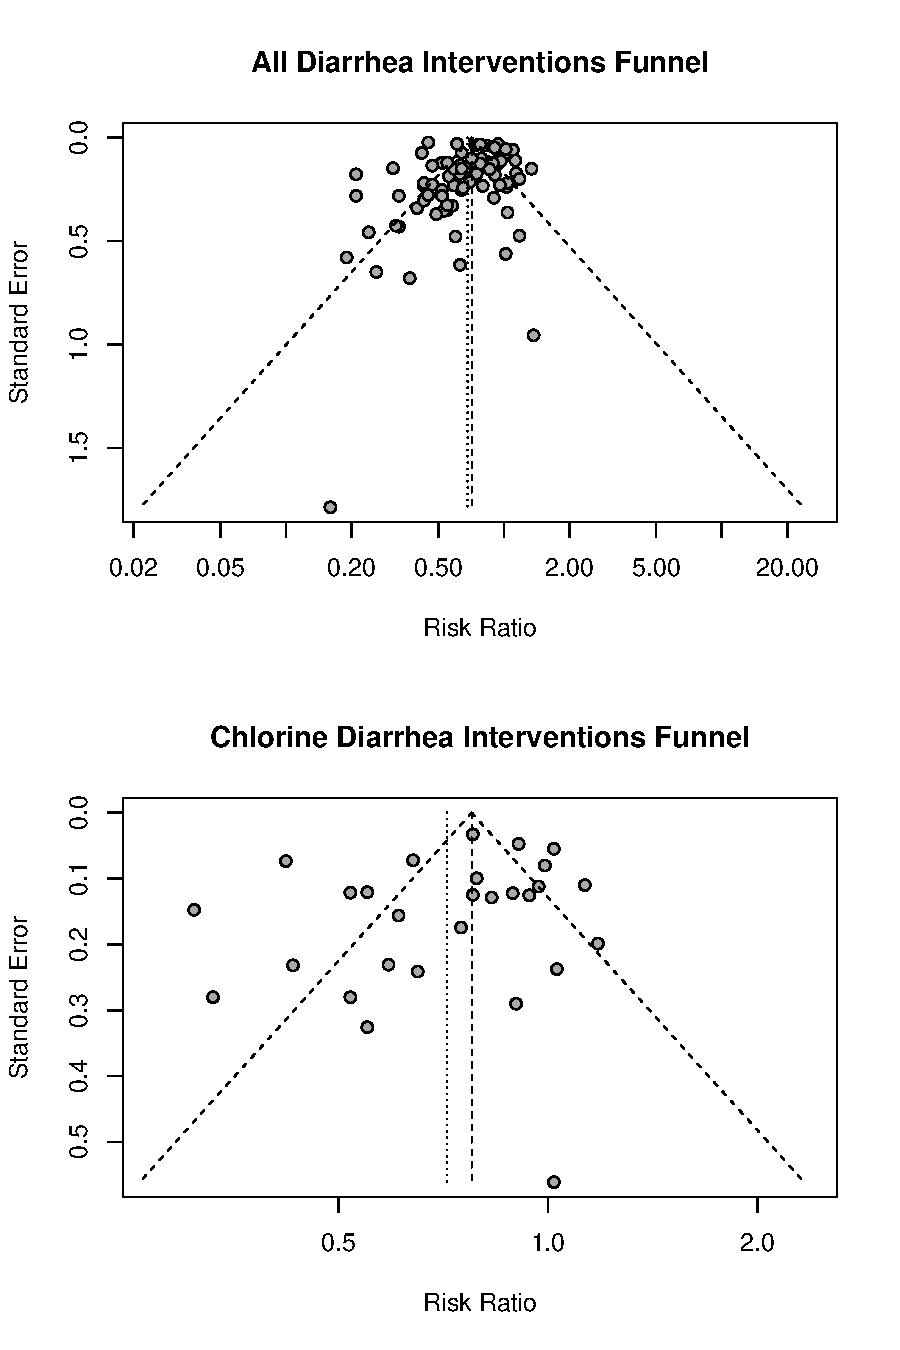
\includegraphics{figures/diarr-pub-bias-funnel.pdf}}
\end{figure}

{\noindent\fontsize{10}{10}\selectfont Notes: Funnel plot to assess publication bias in risk ratio estimates of diarrhea morbidity in all augmented available studies (top panel) and the subset of chlorination studies (bottom panel).}

\newpage
\noindent\textbf{Fig. S5.}  Heterogeneity in treatment effects, by study year
\begin{figure}[H]
    \centering
    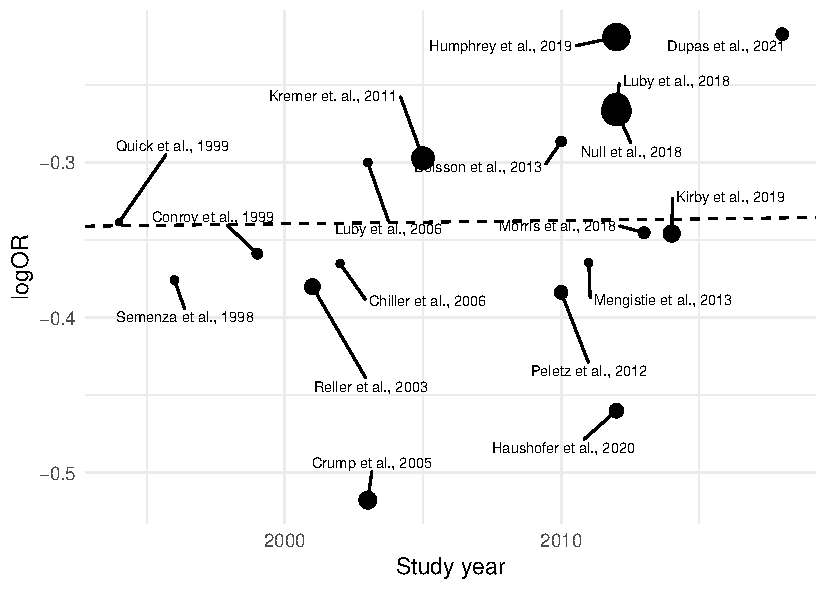
\includegraphics{figures/bubble-plot-year.pdf}
\end{figure}
{\noindent\fontsize{10}{10}\selectfont Notes: The relationship between treatment effect estimates (y axis) and the study year (x axis) across 18 studies included in the sample. Year of intervention is the year that each studied intervention was launched. We find no association (slope is less than 0.0002 per year, with SD = 0.0025) between mortality and study year. Each point represents a study. The size of each bubble is inversely proportional to the standard errors of treatment effect estimate.}



\newpage
\noindent\textbf{Fig. S6.} Diarrhea prevalence in included studies compared to distribution low- and middle- income countries
\begin{figure}[H]
    \centering
    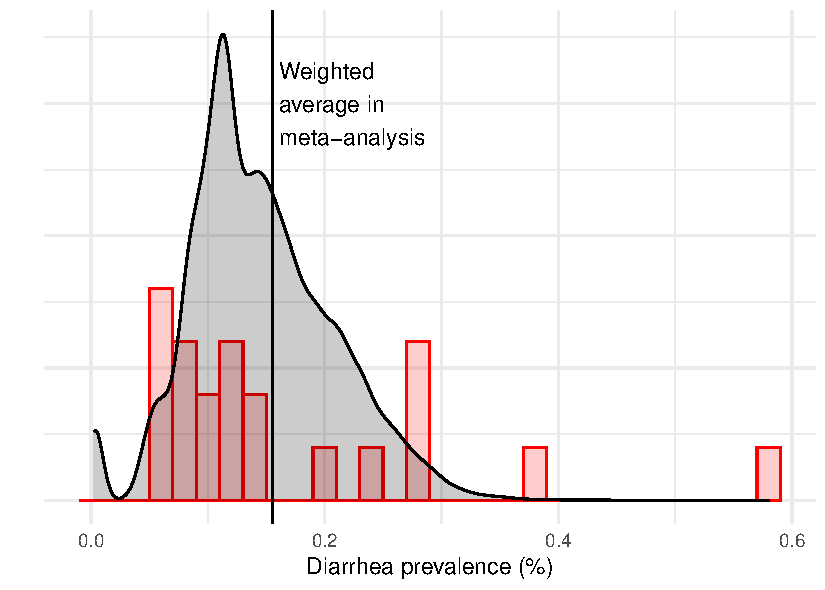
\includegraphics{figures/dist-diarrhea-prevalence.pdf}
\end{figure}

{\noindent\fontsize{10}{10}\selectfont Notes: The gray area represents the density over 43,323 observations of diarrhea prevalence at the sub-national level from 94 countries, based on data from Institute for Health Metrics and Evaluation, 2020. The red histogram is of diarrhea prevalence among the studies included in this meta-analysis. The black bar shows the weighted average of diarrhea prevalence among the studies in the meta-analysis, which is 15.6\%. This corresponds to the 61st percentile of the distribution of sub national diarrhea estimates.}

\newpage
\noindent\textbf{Fig. S7.} Cost-effectiveness as a function of treatment effect
\begin{figure}[H]
    \centering
    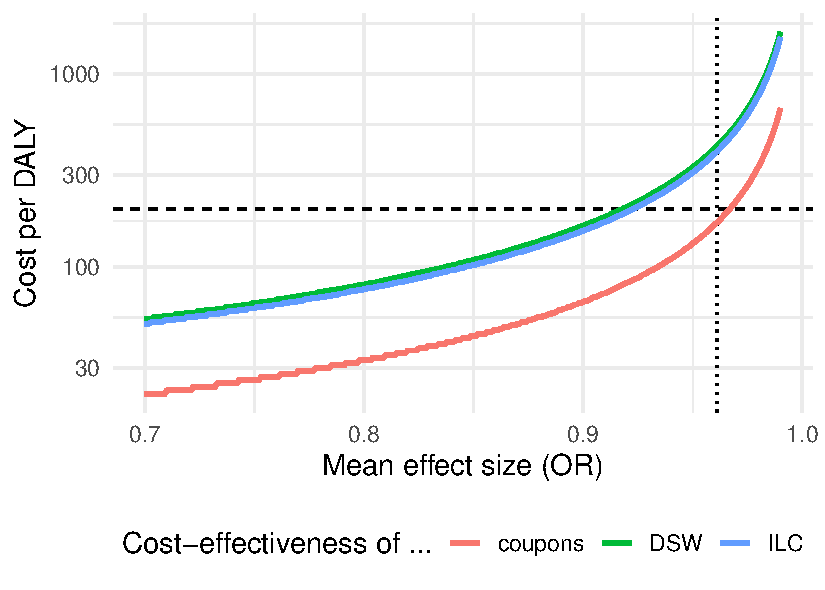
\includegraphics{figures/cea_or_relationship.pdf}
\end{figure}

{\noindent\fontsize{10}{10}\selectfont Notes: The calculation from Table S7 is repeated in this plot, varying the odds ratios on all-cause mortality (X axis) and recalculating USD cost per DALY averted for each of the three methods we investigated. The vertical line corresponds to 0.039 reduction in OR, which we discuss in Section 7 of the supplement. The horizontal line is the most stringent cut-off of 200 USD.}


\end{document}